\subsection{Получение информации о команде c помощью команды info}

\subparagraph{1) Что нужно было сделать?}

То же, что и в п. 5, только с помощью команды info.

\subparagraph{2) Как это сделали?}

\begin{MyVerbatimCode}[label=Debian terminal]
pavel-innokentevich-galanin@aspire-one-725:~$ info ls
\end{MyVerbatimCode}

Результат выполнения команды apropos ls
на~рисунке~\ref{fig:apropos-ls}
(стр.~\pageref{fig:apropos-ls}).

\begin{figure}[!htp]
    \centering
    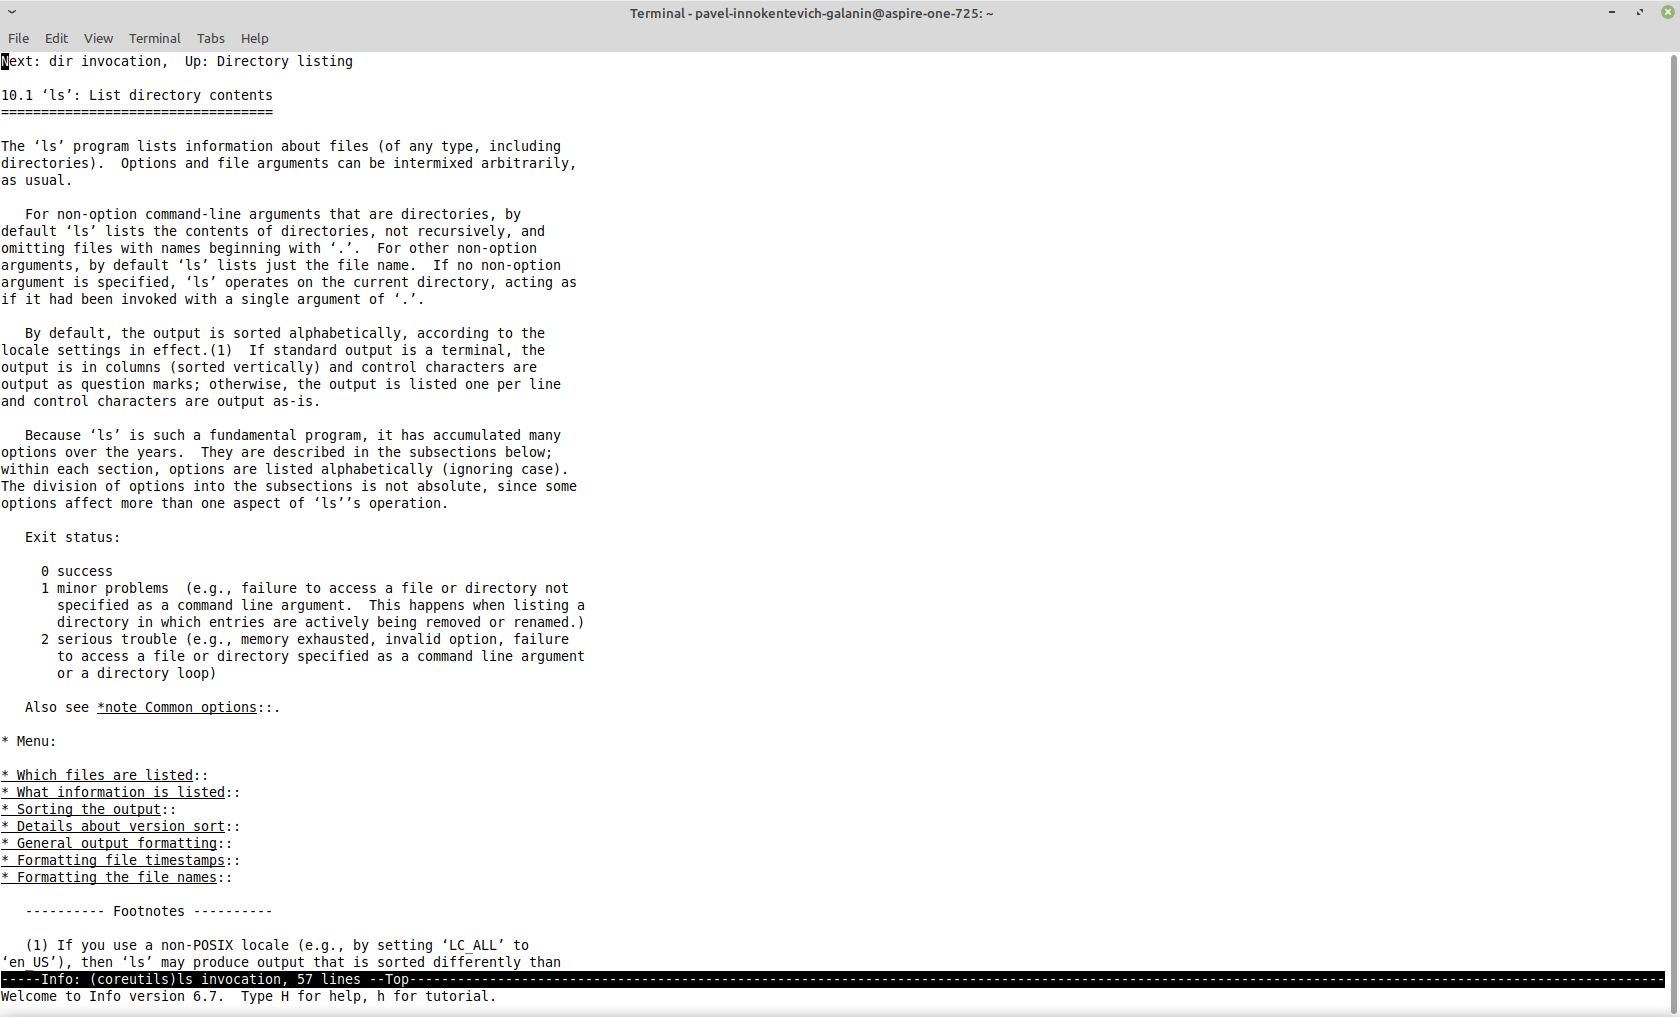
\includegraphics[width=11cm]
        {input/task-1/7/info-ls.png}
    \caption{apropos ls}
    \label{fig:info-ls}
\end{figure}

\begin{MyVerbatimCode}[label=Debian terminal]
pavel-innokentevich-galanin@aspire-one-725:~$ info cd
info: No menu item 'cd' in node '(dir)Top'
\end{MyVerbatimCode}

\subparagraph{3) Что получилось?}

Командой info получили в консоль справочную ифнормацию, если информации нет, то выводится сообщение.
